\chapter{Nouvelles topologies}

On va s'arr�ter un moment afin d'�tudier certaines topologies particuli�res que l'on peut mettre sur un espace vectoriel norm�. Ces topologies sont tr�s particuli�res et leurs propri�t�s diff�rent plus ou moins fortement de la topologie de la norme. Puisque ces topologies sont indispensables � l'�tude des espaces r�flexifs, il est bon d'en apprendre davantage sur celles-ci avant d'aller plus loin. On consid�rera tout au long de ce chapitre des espaces vectoriels norm�s, puisque l'on aura jamais besoin de supposer que l'espace est complet.

\section{Topologie faible}

Soit $E$ un espace vectoriel norm�. Soient $x_0\in E, \varepsilon>0, n\in\mathbb{N}_0, x_1\dual,...,x_n\dual\in E\dual$. On d�finit
\[
V_{\varepsilon, x_1\dual,...,x_n\dual}(x_0)=
\{x\in E~|~\forall k\in\{1,...,n\}, \abs{x_k\dual(x-x_0)}<\varepsilon\}
\]
Le syst�me fondamental de voisinages que l'on d�finit pour $x_0$ est
\[
\{V_{\varepsilon, x_1\dual,...,x_n\dual}(x_0)~|~\varepsilon>0, n\in\mathbb{N}_0, x_1\dual,...,x_n\dual\in E\dual\}
\]
En fait, c'est m�me un syst�me fondamental de voisinages ouverts. En effet, si $x\in V_{\varepsilon, x_1\dual,...,x_n\dual}(x_0)$, alors avec $\delta=\min\limits_{k=1}^n\left(\varepsilon-\abs{x_k\dual(x-x_0)}\right)$, on a que $x\in V_{\delta, x_1\dual,...,x_n\dual}(x)\subseteq V_{\varepsilon, x_1\dual,...,x_n\dual}(x_0)$.

Cette topologie sur $E$ est appel�e topologie faible, et est not�e $\weak{E}$ ou $\omega$.

Pour cette topologie, une suite $(x_n)_{n\in\mathbb{N}}$ � valeurs dans $E$ converge vers $x\in E$ si et seulement si pour toute fonctionnelle $x\dual\in E\dual$, on a $x\dual(x_n)\rightarrow x\dual(x)$.

\begin{center}\begin{tabular}{m{6cm}r}
Voici un exemple de repr�sentation d'un tel voisinage, dans le cas de l'espace $\mathbb{R}^2$ o� on choisit trois application lin�aires.
&
\raisebox{-0.6\height}{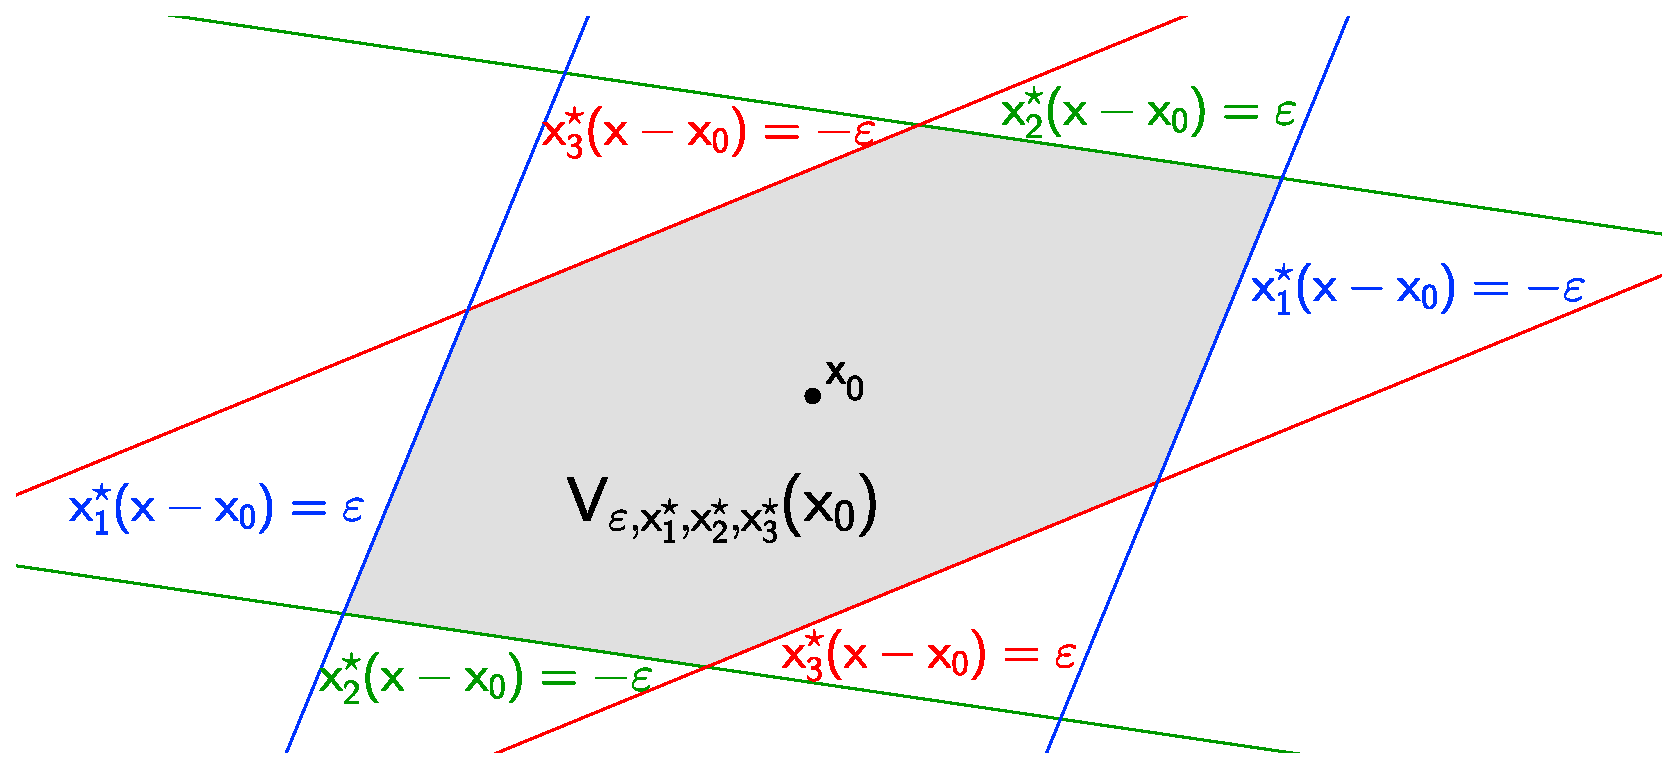
\includegraphics[width = 10.1cm,height=4.9cm]{topo/voisinagefaible.eps}}
\end{tabular}\end{center}

\section{Topologie pr�faible}

Soit $E$ un espace vectoriel norm�. Soient $x_0\dual\in E\dual, \varepsilon>0, n\in\mathbb{N}_0, x_1,...,x_n\in E$. On d�finit
\[
V_{\varepsilon, x_1,...,x_n}(x_0\dual)=
\{x\dual\in E\dual~|~\forall k\in\{1,...,n\}, \abs{(x\dual-x_0\dual)(x_k)}<\varepsilon\}
\]
Le syst�me fondamental de voisinages que l'on d�finit pour $x_0\dual$ est
\[
\{V_{\varepsilon, x_1,...,x_n}(x_0\dual)~|~\varepsilon>0, n\in\mathbb{N}_0, x_1,...,x_n\in E\}
\]
En fait, c'est m�me un syst�me fondamental de voisinages ouverts. On appliquera le m�me raisonnement que pour la topologie faible.

Cette topologie sur $E\dual$ est appel�e topologie pr�faible, et est not�e $\pweak{E}$ ou $\omega\star$.

Pour cette topologie, une suite $(x_n\dual)_{n\in\mathbb{N}}$ � valeurs dans $E\dual$ converge vers $x\dual\in E\dual$ si et seulement si pour tout $x\in E$, on a $x_n\dual(x)\rightarrow x\dual(x)$.

